\documentclass{ximera}

\title{New Coordinate Systems: Polar}
\author{Zack Reed}

\begin{document}
\begin{abstract}
In this activity we explore sets in two and three dimensions, learn about polar coordinates as an alternative coordinate system, and develop skills for working with multivariable functions.
\end{abstract}
\maketitle

\section*{Why Change Coordinate Systems?}

For most of your mathematical career, you've used the Cartesian coordinate system with horizontal $x$-axis and vertical $y$-axis. Points are represented as coordinate pairs $(x,y)$.

\begin{center}
\geogebra{vhyaeqmy}{739}{613}
\end{center}

\begin{problem}
    Using the GeoGebra applet above, drag point $P$ to the location $(3,2)$.
    
    The point $P=(3,2)$ means you move $\answer{3}$ units \wordChoice{\choice[correct]{right}\choice{left}} and $\answer{2}$ units \wordChoice{\choice[correct]{up}\choice{down}} from the origin.
    
    The point $Q=(-1,4)$ means you move $\answer{1}$ unit \wordChoice{\choice{right}\choice[correct]{left}} and $\answer{4}$ units \wordChoice{\choice[correct]{up}\choice{down}} from the origin.

    The point $R=(-1,-3)$ means you move $\answer{1}$ unit \wordChoice{\choice{right}\choice[correct]{left}} and $\answer{3}$ units \wordChoice{\choice[correct]{down}\choice{up}} from the origin.
\end{problem}

\section*{Describing Sets in Cartesian Coordinates}

A \emph{set} is a collection of points $P$. We can describe sets using conditions on $x$ and $y$.

\begin{center}
\geogebra{sucycy28}{689}{563}
\end{center}

\begin{problem}
    Using the GeoGebra applet above, explore the different sets by selecting the checkboxes.
    
    \begin{enumerate}
        \item The rectangular region is described by points $(x,y)$ where $\answer{0} \leq x \leq \answer{3}$ and $\answer{1} \leq y \leq \answer{3}$.
        
        The point $(2,2)$ is \wordChoice{\choice[correct]{inside}\choice{outside}} the rectangular region.

        The point $(4,2)$ is \wordChoice{\choice{inside}\choice[correct]{outside}} the rectangular region.

        The point $(2,0)$ is \wordChoice{\choice{inside}\choice[correct]{outside}} the rectangular region.

        The point $(0,1)$ is \wordChoice{\choice[correct]{inside}\choice{outside}} the rectangular region.
        
        \item The circle is described by the equation $x^2 + y^2 = \answer{1}$.
        
        The point $(0.5,0.5)$ is \wordChoice{\choice[correct]{inside}\choice{on}\choice{outside}} the circle because $0.5^2 + 0.5^2 = \answer{0.5}$ which is \wordChoice{\choice[correct]{less than}\choice{equal to}\choice{greater than}} $1$.

        The point $(\sqrt{2}/2,\sqrt{2}/2)$ is \wordChoice{\choice{inside}\choice[correct]{on}\choice{outside}} the circle because $(\sqrt{2}/2)^2 + (\sqrt{2}/2)^2 = \answer{1}$ which is \wordChoice{\choice{less than}\choice[correct]{equal to}\choice{greater than}} $1$.

        The point $(-1,-1)$ is \wordChoice{\choice{inside}\choice{on}\choice[correct]{outside}} the circle because $(-1)^2 + (-1)^2 = \answer{2}$ which is \wordChoice{\choice{less than}\choice{equal to}\choice[correct]{greater than}} $1$.
        
        \item Set 3 is determined by the $x$ interval $\answer{0} \leq x \leq \answer{1}$ and the $y$ interval $\answer{x^2} \leq y \leq \answer{x}$.
        
        The point $(0.5,0.3)$ is \wordChoice{\choice[correct]{inside}\choice{outside}} Set 3 because $0.5^2 \leq 0.3 \leq 0.5$ is \wordChoice{\choice[correct]{true}\choice{false}}.

        The point $(0.5,0.2)$ is \wordChoice{\choice{inside}\choice[correct]{outside}} Set 3 because $0.5^2 \leq 0.2 \leq 0.5$ is \wordChoice{\choice{true}\choice[correct]{false}}.

        \item While we can see the spiral region and use the applet to explore points in it, describing this set using $x$ and $y$ is quite difficult!
        
        The point $(-4, 2)$ is \wordChoice{\choice[correct]{inside}\choice{outside}\choice{hard to determine whether it is inside or outside of}} the spiral region.

        The point $(-4, 4.5)$ is \wordChoice{\choice{inside}\choice{outside}\choice[correct]{hard to determine whether it is inside or outside of}} the spiral region.
    \end{enumerate}
    
\end{problem}

\section*{Introducing Polar Coordinates}

Instead of describing a point by its horizontal and vertical distances from the origin, we can describe it by:
\begin{itemize}
    \item How far it is from the origin: the radius $r$
    \item What angle we rotate from the positive $x$-axis: the angle $\theta$
\end{itemize}

This gives us polar coordinates $(r,\theta)$.

\begin{center}
\geogebra{r9g6amrn}{691}{563}
\end{center}

\begin{problem}
    Using the polar coordinate GeoGebra applet above, drag point $P$ to explore how $r$ and $\theta$ change.
    
    \begin{enumerate}
        \item When point $P$ is at Cartesian coordinates $(1,0)$, the polar coordinates are $(r,\theta) = (\answer{1},\answer{0})$.
        
        \item When point $P$ is at Cartesian coordinates $(0,1)$, the polar coordinates are $(r,\theta) = (\answer{1},\answer[tolerance=0.01]{\pi/2})$.
        
        %repeat the points from the earlier cartesian problem
        \item When point $P$ is at Cartesian coordinates $(3,2)$, the polar coordinates are $(r,\theta) = (\answer[tolerance=0.01]{3.605},\answer[tolerance=0.01]{.588})$.
        
        \item When point $P$ is at Cartesian coordinates $(-1,4)$, the polar coordinates are $(r,\theta) = (\answer[tolerance=0.01]{4.123},\answer[tolerance=0.01]{1.8215})$.
        
        \item When point $P$ is at Cartesian coordinates $(-1,-3)$, the polar coordinates are $(r,\theta) = (\answer[tolerance=0.01]{3.162},\answer[tolerance=0.01]{4.39})$.
        
        \item As you move $P$ further from the origin, the value of $r$ \wordChoice{\choice[correct]{increases}\choice{decreases}\choice{stays the same}}.
        
        \item As you move $P$ counterclockwise around the origin (at constant distance), the value of $\theta$ \wordChoice{\choice[correct]{increases}\choice{decreases}\choice{stays the same}}.
    \end{enumerate}
\end{problem}

\begin{problem}
    Now let's describe that mysterious fourth set from earlier!
    
    In polar coordinates, the spiral region can be described as:
    \begin{multipleChoice}
        \choice{$r = 2$ and $0 \leq \theta \leq 2\pi$}
        \choice[correct]{$r \leq 2\theta + 1$ and $0 \leq \theta \leq 2\pi$}
        \choice{$\theta = 2r + 1$ and $0 \leq r \leq 2\pi$}
        \choice{$r^2 + \theta^2 = 1$}
    \end{multipleChoice}
    
    \begin{feedback}
        The condition $r \leq 2\theta + 1$ means the radius grows linearly with the angle, creating a spiral! This is much simpler than trying to describe this region using $x$ and $y$.
    \end{feedback}
\end{problem}

\section*{Converting Between Coordinate Systems}

\begin{problem}
    Here are some relationships between Cartesian $(x,y)$ and polar $(r,\theta)$ coordinates that let you efficiently convert between the two systems:
    \begin{align*}
           x = r\cos(\theta), & \text{        } y = r\sin(\theta)  \\
           r = \sqrt{x^2 + y^2}, & \text{        } \theta =\arctan\left(\frac{y}{x}\right)
    \end{align*}

    \begin{center}
    % Diagram 1: circle showing r, x, y triangle
        % Left: Circle with axes
        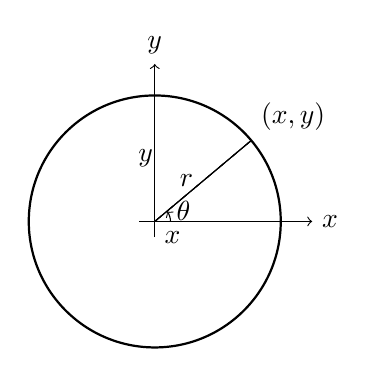
\begin{tikzpicture}[scale=1]
            \def\R{1.6}
            % Axes
            \draw[->] (-0.2,0) -- (2,0) node[right] {$x$};
            \draw[->] (0,-0.2) -- (0,2) node[above] {$y$};
            % Circle
            \draw[thick] (0,0) circle (\R);
            % Point and radius
            \coordinate (P) at (40:\R);
            \draw[dashed] (0,0) -- (P);
            \draw[thin] (0,0) -- (P) node[midway,left] {$r$};
            \draw[thin] (P) -- (40:0) coordinate (X) -- (0,0);
            \draw[->] (0.2,0) arc (0:40:0.2) node[right] {$\theta$};
            \node at (P) [above right] {$(x,y)$};
            \node at (X) [below right] {$x$};
            \node at (0.1,0.8) [left] {$y$};
        \end{tikzpicture}
        \qquad
        % Right: Just the right triangle (no axes/circle)
        \begin{tikzpicture}[scale=1]
            \def\R{1.6}
            \coordinate (A) at (0,0);
            \coordinate (B) at (\R*0.766,0); % x = r cos(theta), y = 0
            \coordinate (C) at (\R*0.766,\R*0.643); % x = r cos(theta), y = r sin(theta)
            \draw[thick] (A) -- (B) -- (C) -- cycle;
            % Angle arc
            \draw[->] (0.25,0) arc (0:40:0.25);
            \node at (0.38,0.08) {$\theta$};
            % Sides
            \node at ($(A)!0.5!(B)$) [below] {$x$};
            \node at ($(B)!0.5!(C)$) [right] {$y$};
            \node at ($(A)!0.5!(C)$) [left] {$r$};
            % Point label
            \node at (C) [above right] {$(x,y)$};
        \end{tikzpicture}
    \end{center}

    \begin{feedback}
        Explanation: Drop a perpendicular from the point $(x,y)$ to the $x$-axis to form a right triangle with legs $x$ (adjacent) and $y$ (opposite) and hypotenuse $r$ (the distance to the origin). By definition of cosine and sine in a right triangle, $\cos(\theta)=\dfrac{x}{r}$ and $\sin(\theta)=\dfrac{y}{r}$. Solving for $x$ and $y$ gives $x=r\cos\theta$ and $y=r\sin\theta$. The unit-circle visualization shows the same idea scaled to $r=1$, where the coordinates on the circle are exactly $(\cos\theta,\sin\theta)$.
    \end{feedback}
\end{problem}

The following video discusses these relationships and conversions in more detail:

\begin{center}
\youtube{7xD7MEdGNCg}
\end{center}

\begin{problem}
    Let's practice converting between coordinate systems.
    
    \begin{enumerate}
        \item Convert the polar coordinates $(r,\theta) = (2, \pi/4)$ to Cartesian coordinates.
        
        $x = \answer[tolerance=0.01]{\sqrt{2}}$ and $y = \answer[tolerance=0.01]{\sqrt{2}}$
        
        \item Convert the Cartesian coordinates $(x,y) = (3,4)$ to polar coordinates.
        
        $r = \answer{5}$ and $\theta = \answer[tolerance=0.01]{\arctan(4/3)}$ radians
        
        \item Convert the polar coordinates $(r,\theta) = (5, 0)$ to Cartesian coordinates.
        
        $x = \answer{5}$ and $y = \answer{0}$
    \end{enumerate}
    
        \begin{feedback}
                Graphical solution for part (2): the point $(3,4)$ forms a right triangle with legs of length $3$ (adjacent) and $4$ (opposite) and hypotenuse $r=5$. Below are two visuals to make this clear.

                \begin{center}
                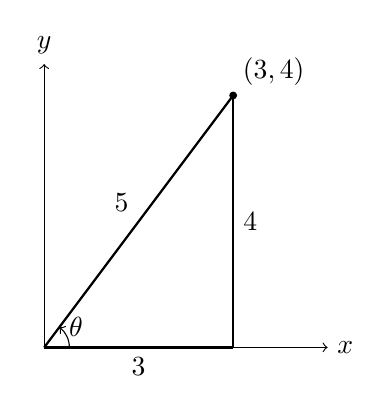
\begin{tikzpicture}[scale=0.8]
                    % axes
                    \draw[->] (0,0) -- (4.5,0) node[right] {$x$};
                    \draw[->] (0,0) -- (0,4.5) node[above] {$y$};
                    % point and projections
                    \coordinate (P) at (3,4);
                    \draw[fill] (P) circle (1.5pt) node[above right] {$(3,4)$};
                    \draw[dashed] (P) -- (3,0) node[midway,right] {} -- (0,0);
                    % triangle sides
                    \draw[thick] (0,0) -- (3,0) node[midway,below] {$3$};
                    \draw[thick] (3,0) -- (3,4) node[midway,right] {$4$};
                    \draw[thick] (0,0) -- (3,4) node[midway,above left] {$5$};
                    % angle
                    \draw[->] (0.4,0) arc (0:53.13:0.4) node[right] {$\theta$};
                \end{tikzpicture}
                \qquad
                \begin{tikzpicture}[scale=0.9]
                    % unit-circle style to show arctan relation
                    \draw[thick] (0,0) circle (1);
                    \coordinate (U) at (0.6,0.8); % same slope 4/3 scaled
                    \draw[fill] (U) circle (1.5pt) node[above right] {direction};
                    \draw[dashed] (U) -- (0.6,0) node[midway,below] {$\dfrac{3}{5}$} -- (0,0);
                    \node at (0.35,0.45) [right] {$\dfrac{4}{5}$};
                    \draw[->] (0.2,0) arc (0:53.13:0.2) node[right] {$\theta$};
                \end{tikzpicture}
                \end{center}

                Calculation: $r=\sqrt{3^2+4^2}=5$. The angle satisfies $\tan\theta=\dfrac{4}{3}$, so $\theta=\arctan(4/3)$ (adjusted for quadrant if needed). Thus the polar coordinates are $(5,\arctan(4/3))$.
        \end{feedback}
\end{problem}

\end{document}